% -*- root: ../../main.tex -*- %
- image = activity/workflow, container = activity instance / workflow instance

There are several possibilities how Docker can be utilized for the execution of workflows.
Each combination of variants (abbreviated as depicted in Table~\ref{tab:docker_variants}) has its own advantages and disadvantages, which are elaborated in this chapter.

The first aspect is whether one wants to spread the containers associated with one workflow instance across various machines for execution ($S$) or constraint them to run on the same node as a group ($G$).

Second, one can differentiate to which extend workflow components are wrapped in their own containers.
One could encapsulate only activities in containers ($*_{AC}^{*}$) and distribute workflow information on another way, let each workflow and activity reside in a different container ($*_{SEPC}^{*}$), or wrap them in one container together ($*_{1C}^{*}$). Since this container is an atomic unit, it cannot be spread across many nodes for execution. One also could abandon the idea of a one-to-one mapping between the Docker and workflow concepts and establish worker containers with specialized behavior (according to a workflow/activity type) which perform suitable tasks on request ($*_{Type}^{*}$).

Third, it is important to define the way data is exchanged between containers. One possible solution could be a data volume that is shared by all containers in need to exchange data with each other ($*_{*}^{DV}$). Data could also be passed between containers via some system service, \eg a database, ($*_{*}^{SER}$), or on a direct connection between the containers ($*_{*}^{D}$).

Finally, rather independent from the previous variants and hence discussed in isolation, one might want to choose the mechanism that decides which containers are run on which machines, \ie the execution scheduling.

TODO: table consistent with text?

\begin{table}[!htbp]
  \centering
  %\renewcommand*{\arraystretch}{1.25}
  \begin{tabular}{C{4cm}|C{3cm}|C{3cm}|C{3cm}}
    \toprule
    \textbf{Data Exchange / Containerization}

    & Common Data~Volume  & Service & Direct \\ \midrule

    \multicolumn{4}{c}{\textbf{Grouped execution on one node} }\\ [1ex] \midrule

    Activities in containers
    & $G_{AC}^{DV}$   & $G_{AC}^{SER}$  & $G_{AC}^{D}$   \\ \midrule

    Workflows and activities in separate containers
    & $G_{SEPC}^{DV}$  & $G_{SEPC}^{SER}$ & $G_{SEPC}^{D}$  \\ \midrule

    Workflow and activities in one container
    & $G_{1C}^{DV}$  & $G_{1C}^{SER}$ & $G_{1C}^{D}$  \\ \midrule

    Type based workers
    & $G_{Type}^{DV}$  & $G_{Type}^{SER}$ & $G_{Type}^{D}$  \\ \midrule

    \multicolumn{4}{c}{\textbf{Spread execution over available nodes} }\\ [1ex] \midrule

    Activities in containers
    & \xmark & $S_{AC}^{SER}$ & $S_{AC}^{D}$ \\ \midrule

    Workflows and activities in separate containers
    & \xmark & $S_{SEPC}^{SER}$ & $S_{SEPC}^{D}$ \\ \midrule

    Workflow and activities in one container
    & \xmark & \xmark & \xmark \\ \midrule

    Type based workers
    & \xmark & $S_{Type}^{SER}$ & $S_{Type}^{D}$ \\ \midrule

    \bottomrule
  \end{tabular}
  \caption{Containerization/Grouping/Communication Solution Pairings}
  \label{tab:docker_variants}
\end{table}

\subsection{Mode of operation of the Aspects} % (fold)
\label{sub:mode_of_operation_of_the_aspects}
  **ASD ASD ASD** (afrob und samy deluxe)
  In the following the previously introduced concepts are explained in more detail and some variations on them are given.

  \subsubsection{Grouped or spread execution} % (fold)
  \label{ssub:grouped_or_spread_execution}
    - couple all containers
    - couple specific containers
    - spread execution
  % subsubsection grouped_or_spread_execution (end)

  \subsubsection{Element-wrapping containers} % (fold)
  \label{ssub:element_wrapping_containers}
    - functionality in image layers
    - instance specifics in container write layer
    - started / ended

    \begin{figure}[htbp]
      \centering
      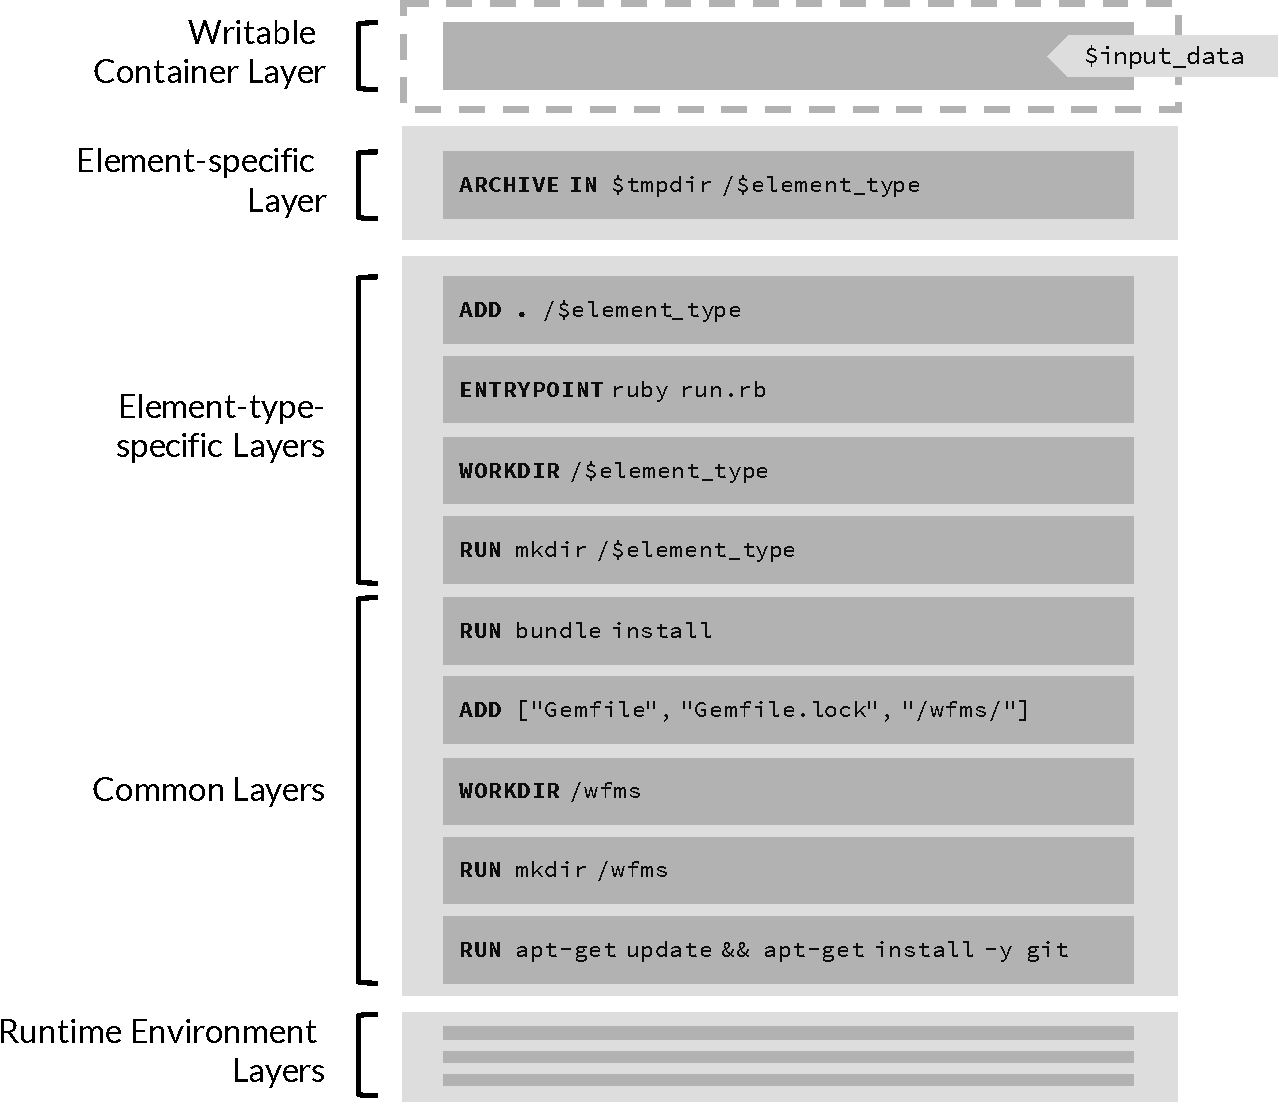
\includegraphics[width=0.95\textwidth]{content/images/execution_container-crop.pdf}
      \caption{Layer Contents for Element-wrapping Containers}
      \label{fig:layers_for_element_wrapping_containers}
    \end{figure}

    \begin{figure}[htbp]
      \centering
      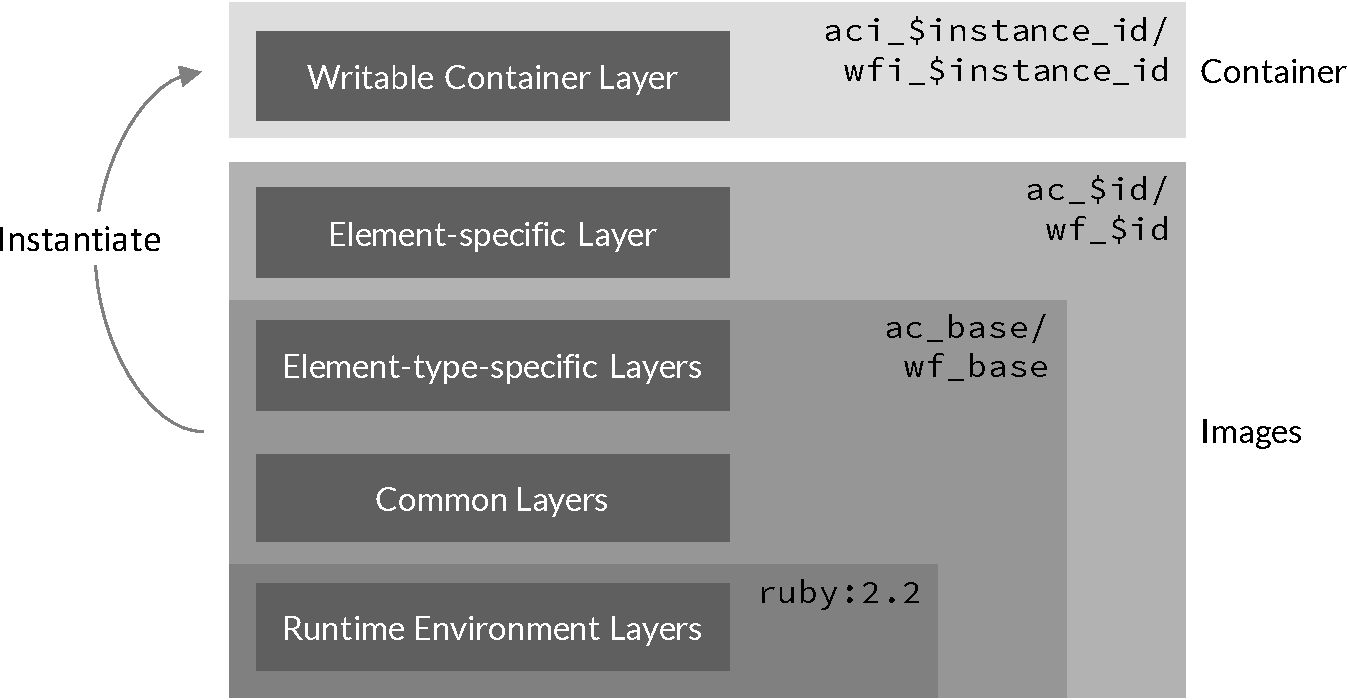
\includegraphics[width=0.95\textwidth]{content/images/layer_concept-crop.pdf}
      \caption{Layers of Element-wrapping containers}
      \label{fig:layers_for_element_wrapping_containers}
    \end{figure}
  % subsubsection element_wrapping_containers (end)

  \subsubsection{Worker containers} % (fold)
  \label{ssub:worker_containers}
    - generic functionality in image layers
    - instance specifica passed in
    - keeps running
  % subsubsection worker_containers (end)

  \subsubsection{Data Exchange via Data Volume} % (fold)
  \label{ssub:data_exchange_via_data_volume}

    The idea behind this concept is, that all containers involved in the execution of one workflow instance have access to a common working directory, in which the data visibility scopes can be established using a file system structure. This working directory resides in a data volume owned by a container that is specific to the respective workflow instance and whose only purpose is to ensure the existence of said volume.

    - data volume mountable via -v option
    - arbitrary name and location in container

    - structure
      - simple
        - self-managed by all participating containers (/tmp)
      - predefined
        - env/wf\_/wc\_ for data defined at build time
        - wfi\_ for current workflow instance
          - nested aci\_/wfi\_ for child elements
        - as in Figure~\ref{fig:dv_dir_structure}
    - access
      - mount respective workdir as wrd
        - copy/ link required data
      - mount root workdir and pass own workdir name
        - directly access required data

    \begin{figure}[htbp]
      \centering
      \begin{forest}
        dir tree
        [workflow\_relevant\_data
          [env]
          [wf\_1cc594ba-...]
          [wf\_b45d2564-...]
          [ac\_0225d86f-...]
          [ac\_2a5aa4ff-...]
          [ac\_7fc09132-...]
          [wfi\_e65c8533-... \textcolor{gray}{(instance of wf\_1cc594ba-...)}
            [aci\_76b8680c-... \textcolor{gray}{(instance of ac\_0225d86f-...)}]
            [aci\_1e09d287-... \textcolor{gray}{(instance of ac\_2a5aa4ff-...)}
              [wfi\_68e17268-... \textcolor{gray}{(instance of wf\_b45d2564-...)}
                [aci\_2708fd1a-... \textcolor{gray}{(instance of ac\_7fc09132-...)}]
              ]
            ]
          ]
        ]
      \end{forest}
      \caption{Exemplary directory structure for $G_{*}^{DV}$}
      \label{fig:dv_dir_structure}
    \end{figure}
  % subsubsection data_exchange_via_data_volume (end)

  \subsubsection{Data Exchange via Service} % (fold)
  \label{ssub:data_exchange_via_service}
    - communication via MOM
    -
  % subsubsection data_exchange_via_service (end)

  \subsubsection{Data Exchange via Direct Communication} % (fold)
  \label{ssub:data_exchange_via_direct_communication}
    - communidation via REST / Sockets
  % subsubsection data_exchange_via_direct_communication (end)
% subsection mode_of_operation_of_the_aspects (end)


\subsection[Grouped execution using common data volume]{Grouped execution using common data volume ($G_{*}^{DV}$)} % (fold)
\label{sub:grouped_execution_using_common_data_volume}

  $G_{*}^{DV}$ natively supports all identified types of data visibility by providing respective directories and access to them, with the limitation that workflow data and environment data has to be copied to the data volume before execution and is thus restricted to the state it had at that time. Altering this data is possible, \eg by replacing the respective files via \texttt{docker copy} or altering it in a \texttt{docker exec} session, but extra measures have to be taken to request such an up-to-date version.

  Data interactions between activity instances, a sub-workflow activity and its related components and vice versa are supported by $G_{*}^{DV}$. Exchanging data between two running workflow instances is not possible, though, as mounting volumes to running containers is not supported by Docker yet. This kind of interaction thus requires some additional tools. It would be possible to grant access to workflow instances running on the same machine -- at the price of loss of control over data visibility -- by mounting the top-level working directory of that machine in all containers.

  As long as no requests to external sources are made within the workflow, data has to be transferred over the network only twice in this approach -- for the input and output of the workflow. All subsequent data transfers are either implicit, \eg by accessing the respective working directory or a symbolic link to it, or take place on the local machine, \eg copying one or more files. Because of transfer rates *QUOTE*, $G_{*}^{DV}$ has an advantage over message-based approaches when it comes to processing of large and/or many data sets, \ie log files, genome research data or images. Also, unless required by the activities themselves, data conversion is less of an issue since relying on the file system allows arbitrary file types to be used.

  Sharing a data volume using only Docker tools requires all containers to be on the same machine, which is why there is no spread version $S_{*}^{DV}$ of this concept. Approaches exist to utilize \ac{NFS} or \ac{P2P} file sharing for distributed access to data volumes, but given the limited scope of this thesis they shall not be regarded further here \cite{Miell2015How}.

  $G_{1C}^{DV}$ could theoretically work on its own file system in the editable layer of the container without a dedicated data volume, since all workflow components would have access to it. This would make the container self contained on the one hand -- and thus easier to export or migrate -- but would on the other hand couple the data life cycle to the processing container's life cycle. That is, if the container is removed, the data is removed with it.

% subsection grouped_execution_using_common_data_volume (end)

\subsection[Grouped or spread execution using an intermediate service]{Grouped or spread execution using an intermediate service ($G_{*}^{SER}$ /$s_{*}^{SER}$)} % (fold)
\label{sub:grouped_execution_using_a_intermediate_service}

  $*_{*}^{SER}$ represents the concept of providing some service that is able to store and serve data on request. This implies, that the docker containers have to feature a mechanism to communicate to this service.

  The service could either be running as a single instance on some node in the network or on each node in the network. While the former avoids having to deal with synchronization between service instances and inconsistencies resulting from race conditions, the latter could balance the load. (shorten repsonse times? hops)

  Since the storage of workflow related data is decoupled from the execution in $*_{*}^{SER}$, the coverage of data visibility and data interaction capabilities depends on the chosen underlying service. Theoretically, all forms of data visibility and interactions should thus be possible. Also, the solution exhibits the same properties for the grouped and spread execution, for the same reason.

  In this variant, data is transferred before and after each step in the workflow, \ie when the execution starts, when it ends, whenever an activity is instantiated or an instance finished its work. This is only economical if the amount of data is sufficiently small or if the workflows consist of few activities.

  In order for the workflow execution to function correctly, the service must be reliably available to all containers.

  - service must be present

  - think about hosting multiple services (1 per node)
  - probably superfluous network roundtrip
  - less efficient for large files than using a file system

% subsection grouped_execution_using_a_intermediate_service (end)

\subsection[Grouped or spread execution using direct connections]{Grouped or spread execution using direct connections ($G_{*}^{D}$/$S_{*}^{D}$)} % (fold)
\label{sub:grouped_execution_using_direct_connections}

  In this scenario, the containers communicate with each other directly in order to exchange workflow relevant data. It can be split again in two sub-variants, according to the data passing patterns noted in \ref{sub:workflow_data}. On the one hand, one where the workflow relevant data is passed along the control flow ($*_{*}^{D_j}$). On the other hand, one where containers can query each other for their data($*_{*}^{D_s}$).

  \subsubsection{Joined data and control flows ($*_{*}^{D_j}$)} % (fold)
    In $*_{*}^{D_j}$, the data flow is is directly coupled to the control flow, \ie all data is passed on on invocation. This requires all data that might be used in another activity instance to be passed along, no matter whether the succeeding activity uses them or not \cite{Russell2005Workflow}. While this allows to pass (and update) workflow and environment data, it may be problematic for larger amounts of data.
  % subsubsection ___d_a_ (end)

  \subsubsection{Separate data and control flows ($*_{*}^{D_s}$)} % (fold)
    $*_{*}^{D_s}$ requires all containers that shall be queried for data to provide some communication mechanism and to be running. Thus, in the worst case every container related to a workflow instance has to be running. Even though the containers' use of processor time can be reduced by pausing them until they are needed, this approach could impose a considerable strain on the host machine's memory, as pausing containers has no effect on their memory consumption.

    Workflow data and environment data in $*_{*}^{D_s}$ may be provided to the first activity, which then could be queried for a (static) version of it. Because workflow instances are not represented as containers in $*_{AC}^{D}$, $*_{AC}^{D_s}$ provides no means to store and access sub-workflow data, multiple instance data and workflow instance data.

    $*_{Type}^{D_s}$ is not a feasible solution, as keeping the worker containers running in order to make them queryable would block their use for other workflow instances, thus rendering the \ac{WfMS} incapable of processing further workflow instances once all workers are invoked -- unless further workers are spawned.
  % subsubsection (end)

  As all workflow components reside in one container in $G_{1C}^{D}$, no communication between containers is necessary -- all data can be exchanged on an arbitrary way within that single container. This variant thus represents a special case.
% subsection grouped_execution_using_direct_connections (end)

\begin{table}[!htbp]
  \centering
  %\renewcommand*{\arraystretch}{1.7}
  \begin{tabular}{C{1cm} C{1cm} C{1cm} C{1cm} C{1cm} C{1cm} C{1cm} | C{1cm} C{1cm} C{1cm} C{1cm}}
    \toprule

    \multicolumn{6}{c}{Data Visibility} & \multicolumn{4}{c}{Data Interactions} \\

      & \rot{Ac Data}
      & \rot{SubWF Ac Data}
      & \rot{MultInst Ac Data}
      & \rot{WFInst Data}
      & \rot{WF Data}
      & \rot{Env Data}

      & \rot{Ac $\rightarrow$ Ac}
      & \rot{SubWF Ac $\rightarrow$ SubWF}
      & \rot{SubWF $\rightarrow$ SubWF Ac}
      & \rot{WFInst $\rightarrow$ WFInst}
    \\ \midrule


                    % A Data   | SWF A Data       | Mult. Inst. A D  | Wf. Instance D   | Wf. Data        | Environment Da || AC -> AC         | subwf a -> subwf | subwf -> subwf a | wfi -> wfi

    $G_{AC}^{DV}$    & \ja     & \ja              & \ja              & \ja              & \ja ($\dagger$) & \ja ($\dagger$) & \ja              & \ja              & \ja              & $\bigcirc$      \\ \midrule
    $G_{SEPC}^{DV}$  & \ja     & \ja              & \ja              & \ja              & \ja ($\dagger$) & \ja ($\dagger$) & \ja              & \ja              & \ja              & $\bigcirc$      \\ \midrule
    $G_{1C}^{DV}$    & \ja     & \ja              & \ja              & \ja              & \ja ($\dagger$) & \ja ($\dagger$) & \ja              & \ja              & \ja              & $\bigcirc$      \\ \midrule
    $G_{Type}^{DV}$  & \ja     & \ja              & \ja              & \ja              & \ja ($\dagger$) & \ja ($\dagger$) & \ja              & \ja              & \ja              & $\bigcirc$      \\ \midrule

    $G_{AC}^{SER}$   & \ja     & \ja              & \ja              & \ja              & \ja             & \ja             & \ja              & \ja              & \ja              & \ja             \\ \midrule
    $G_{SEPC}^{SER}$ & \ja     & \ja              & \ja              & \ja              & \ja             & \ja             & \ja              & \ja              & \ja              & \ja             \\ \midrule
    $G_{1C}^{SER}$   & \ja     & \ja              & \ja              & \ja              & \ja             & \ja             & \ja              & \ja              & \ja              & \ja             \\ \midrule
    $G_{Type}^{SER}$ & \ja     & \ja              & \ja              & \ja              & \ja             & \ja             & \ja              & \ja              & \ja              & \ja             \\ \midrule

    $G_{AC}^{D_j}$   & \ja     & \ja              & $\bigcirc$       & \ja              & \ja             & \ja             & \ja ($\ddagger$) & $\bigcirc$       & $\bigcirc$       & $\bigcirc$      \\ \midrule
    $G_{AC}^{D_s}$   & \ja     & $\bigcirc$       & $\bigcirc$       & $\bigcirc$       & $\bigcirc$      & $\bigcirc$      & \ja ($\ddagger$) & $\bigcirc$       & $\bigcirc$       & $\bigcirc$      \\ \midrule
    $G_{SEPC}^{D}$   & \ja     & \ja ($\ddagger$) & \ja ($\ddagger$) & \ja ($\ddagger$) & $\bigcirc$      & $\bigcirc$      & \ja ($\ddagger$) & \ja ($\ddagger$) & \ja ($\ddagger$) & \ja ($\ddagger$)\\ \midrule
    $G_{1C}^{D}$     & \ja$^*$ & \ja$^*$          & \ja$^*$          & \ja$^*$          & $\bigcirc$      & $\bigcirc$      & \ja$^*$          & \ja$^*$          & \ja$^*$          & \ja$^*$         \\ \midrule
    $G_{Type}^{D}$   & \ja     & \ja ($\ddagger$) & \ja ($\ddagger$) & \ja ($\ddagger$) & $\bigcirc$      & $\bigcirc$      & \ja ($\ddagger$) & \ja ($\ddagger$) & \ja ($\ddagger$) & \ja ($\ddagger$)\\ \midrule

    $S_{AC}^{SER}$   & \ja     & \ja              & \ja              & \ja              & \ja             & \ja             & \ja              & \ja              & \ja              & \ja             \\ \midrule
    $S_{SEPC}^{SER}$ & \ja     & \ja              & \ja              & \ja              & \ja             & \ja             & \ja              & \ja              & \ja              & \ja             \\ \midrule
    $S_{Type}^{SER}$ & \ja     & \ja              & \ja              & \ja              & \ja             & \ja             & \ja              & \ja              & \ja              & \ja             \\ \midrule

    $S_{AC}^{D}$     & \ja     & $\bigcirc$       & $\bigcirc$       &  $\bigcirc$      & $\bigcirc$ & $\bigcirc$  & \ja ($\ddagger$) & $\bigcirc$       & $\bigcirc$       & $\bigcirc$      \\ \midrule
    $S_{SEPC}^{D}$   & \ja     & \ja              & \ja              & \ja              & $\bigcirc$ & $\bigcirc$  & \ja ($\ddagger$) &\ja ($\ddagger$)  & \ja ($\ddagger$) &\ja ($\ddagger$) \\ \midrule
    $S_{Type}^{D}$   & \ja     & \ja              & \ja              & \ja              & $\bigcirc$ & $\bigcirc$  & \ja ($\ddagger$) &\ja ($\ddagger$)  & \ja ($\ddagger$) &\ja ($\ddagger$) \\ \bottomrule
  \end{tabular}
  \captionsetup{justification=centering}
  \caption*{\ja~ natively supported ~~|~~ \ja$^*$~ natively supported, a direct connection within the container is assumed ~~|~~ \ja ($\dagger$)~ can be passsed on instantiation, real-time access requires additional tools \\ \ja ($\ddagger$) natively supported, assuming that all containers are left running for the time of workflow execution ~~|~~ $\bigcirc$~ not natively supported, requires additional tools \\[1em]

  Ac = Activity ~|~ SubWF = Sub-workflow~|~ MultInst = Multiple instance ~|~ WFInst = Workflow instance~|~ WF = Workflow ~|~ Env = Environment
  }
  \label{tab:docker_variants}
  \caption{Containerization/Grouping/Communication Solution Pairings}
\end{table}

\subsection{Promising combinations of characteristics} % (fold)
\label{sub:promising_combinations_of_characteristics}
  Due to its shortcomings regarding the supported types of data visibility and interactions, direct communication between instance-related containers ($*_{*}^{D}$) can be ruled out as a candidate for the prototype. The remaining combinations may be eligible depending on the intended use case and desired properties of the \ac{WfMS}, \eg the kind of data that is processed, the targeted infrastructure, and nature of the workflows.

  If the data volume approach is chosen, one is committed to grouped execution on one node. Considering the different containerization solutions, $G_{SEPC}^{DV}$ is favorable over $G_{AC}^{DV}$, because the explicit existence of containers which represent (sub-)workflow instances makes it possible to both track their state using Docker mechanisms and manage their respective working directories. Embedding workflow engine logic into these containers could enable workflows to be exported and used in a stand-alone fashion.

  $G_{SEPC}^{DV}$ is also favorable over $G_{1C}^{DV}$, because the modularity of $G_{SEPC}^{DV}$ permits to update single activities within the workflow by distributing new versions of their respective image. In $G_{1C}^{DV}$, the whole image would have to be updated due to the way layering in Docker images works. Also, $G_{1C}^{DV}$ does not provide the means to track the activity instances' life cycles with Docker mechanisms, only that of the workflow instance. If the workflow is not meant to be updated but to be distributed to third parties as a stand-alone solution, \eg an automated batch process for photos that is sold to photographers, it is a viable option, though.

  The main benefit of $*_{Type}^{*}$ is that it allows to distribute the workload among several workers. Since $G_{*}^{DV}$ requires all involved workers to be on the same machine, this advantage is voided.

  Altogether, this makes $G_{SEPC}^{DV}$ the variant of choice for data-centric \acp{WfMS}.

  When comparing the service-based variants with each other, $G_{*}^{SER}$ and $S_{*}^{SER}$ share most their advantages and drawbacks. $S_{*}^{SER}$ permits the containers to run on different nodes, though. As this allows containers to be assigned to machines according to their resource requirements and the momentary workload of a machine, it is the preferred variant of those two.

  Because the decoupling of data and containers is well supported by $*_{*}^{SER}$, it is a good fit for the worker-based approach of $*_{TYPE}^{*}$, which in turn facilitates load balancing.

    - AC vs SEPC?

  ** DECISION TREE**
% subsection promising_combinations_of_characteristics (end)


\subsection{Execution Scheduling} % (fold)
\label{sub:execution_scheduling}
  In the course of a workflow enactment, several containers have to be instantiated -- unless the worker-based approach ($*_{TYPE}^{*}$) is chosen. Choosing the node on which the instantiation takes place is a task that may impact the performance of the containers and the enactment itself, as the nodes may differ regarding their available resources. There are three aspects that concern the scheduling of containers: whether Docker Swarm or a custom component manages it, by which rules or criteria the scheduling takes place, and whether and how the user should be able to take influence on the scheduling.

  \subsubsection{Identification of Desired Scheduling Criteria} % (fold)
  \label{ssub:identification_of_desired_scheduling_criteria}
    In order to examine scheduling solutions, some goals should be specified to which they can be evaluated against -- an exhaustive list of these goals is not in the scope of this thesis, though. Thus, two groups of scheduling goals are considered.

    On the one hand, scheduling may be performed based on the properties of the nodes, which can be of qualitative or quantitative nature. Examples for qualitative node properties could be its name, geographical location, membership in some arbitrary grouping, the intended use

    On the other hand, containers may be assigned to nodes based on \ac{WfMS}-specific data.

    - scheduling goals
      - based on WFMS info
        - active components
        - internal data
        - nature of activity/workflow
      - based on node resources
        - qualitative
        - quantitative

    \begin{table}[!htbp]
      \centering
      \begin{tabular}{r c c}
        \toprule
        \textbf{Scheduling based on} & Docker Swarm & Custom Component \\
        \midrule
        \textbf{Node Properties} & \cmark & \cmark \\
        Qualitative & \cmark & \cmark \\
        Quantitative & \cmark & \cmark \\ \midrule
        \textbf{\ac{WfMS} Data} & \cmark & \cmark\\
        Live Data & \xmark & \cmark \\
        Active Workflow Components  & $\bigcirc$ & \cmark \\
        Activity/Workflow Properties & \cmark & \cmark \\
        \bottomrule
      \end{tabular}
      \label{tab:scheduling_criteria}
      \captionsetup{justification=centering}
      \caption*{\footnotesize{\ja~ supported ~~|~~ $\bigcirc$~ depends on chosen containerization model, (partially supported for $*_{*}^{AC}$/$*_{*}^{SEPC}$) ~~|~~ \xmark~ not supported}
      }
      \caption{Supported Scheduling Criteria}
    \end{table}
  % subsubsection identification_of_desired_scheduling_criteria (end)

  \subsubsection{Scheduling Abilities of Docker Swarm} % (fold)
    \label{ssub:abilities_of_docker_swarm}
    As mentioned in \ref{sub:docker_swarm}, Docker Swarm offers two kinds of scheduling mechanisms: filters and strategies. Filters can be passed on instantiation as an environment variable parameter with the format \texttt{<filter-type>:<key><operator><value>}. The value of \texttt{filter-type} can either be ``constraint'' or ``affinity'' -- the two types of filters supported by Swarm.

    \texttt{<key>} can take the values \emph{node} or \emph{container} (which signals a comparison to the respective name or \ac{ID}), one of the default node tags, or the name of some custom label which can refer to both node labels and container labels. By default, nodes get tagged by Docker with a name, their \ac{ID}, their storage driver, their execution driver, the kernel version they use and the name of their operating system.
    Custom labels may be applied to nodes when their daemon is started and to containers as a parameter to the \texttt{run} command. In order to avoid conflicting label names, reverse domain name notation is advised by Docker.
    \texttt{<operator>} may either take the value \texttt{==} or \texttt{!=}, indicating whether a match is desired or should be avoided. It can be followed by a tilde, \eg \texttt{==~} to signal that if the condition cannot be met, the container should be scheduled according to a strategy instead.
    The \texttt{<value>} is a string made of alpha-numeric characters, dots, hyphens, and underscores. It may be either a regular expression or a globbing pattern, to which names, \acp{ID} tags or labels will be matched against.

    Constraints focus on the characteristics of nodes for scheduling; either \ref{itm:const_first} some identifier or \ref{itm:const_second} node tags or \ref{itm:const_third} labels:

    \begin{enumerate}[label=\alph*), nosep]
      \item \label{itm:const_first} \texttt{constraint:node==...}
      \item \label{itm:const_second} \texttt{constraint:operatingsystem==...}
      \item \label{itm:const_third} \texttt{constraint:com.example.label==...}
    \end{enumerate}

    Affinities can be specified to schedule containers based on the presence of images or containers on the target node. Possible criteria are \ref{itm:aff_first} container names or \acp{ID}, \ref{itm:aff_second} image names or \acp{ID} or \ref{itm:aff_third} a custom label on a container:

    \begin{enumerate}[label=\alph*), nosep]
      \item \label{itm:aff_first} \texttt{affinity:container==...}
      \item \label{itm:aff_second} \texttt{affinity:image==...}
      \item \label{itm:aff_third} \texttt{affinity:com.example.label==...}
    \end{enumerate}

    Further, there are some implicit forms of scheduling. First, containers will not be executed on nodes that Swarm considers \emph{unhealthy}, \ie that do not respond or otherwise exhibit faulty behavior. Second, some Docker features imply scheduling rules. If the container requires an exposed port, it will not be scheduled on nodes where this port is already occupied. Mounted volumes of, a shared network stack with or a link to another container imply an affinity to that container, which will prohibit the execution if it is not met.
  % subsubsection abilities_of_docker_swarm (end)

  \subsubsection{Abilities of Custom Scheduling Components} % (fold)
  \label{ssub:abilities_of_custom_scheduling_components}
    By querying the swarm master, a custom scheduler component can theoretically infer the information required to perform the same kind of scheduling offered by Docker Swarm. Opposed to the latter, it could further acquire information related to current workflow enactments and perform the scheduling based on that live data. For example, if an user specifies his/her current location in the course of a workflow enactment, all subsequent containers could be scheduled to run on nodes that suit the laws of that country.
  % subsubsection abilities_of_custom_scheduling_components (end)

  \subsubsection{Approaches for Scheduling Criteria} % (fold)
  \label{ssub:approaches_for_scheduling_criteria}
    - swarm
      - docker based
        - qualitative: encode in labels
        - quantitative: encode in labels
      - wfms based
        - Live Data
          - no, cannot man
        - Active Workflow Components
          - get running containers, rules based on container labels
        - ``passive'' Activity/Workflow Properties
          - encode in labels
    - custom
      - like swarm

    - solutions
      - container state (wf status based)
        - only custom solution
      - location based (eg for compliance)
        - label
        - ip?
      - resource based
        - regex for comparisons
          - eg
            - label: wfms.ram.\$ram in mb
            - \texttt{wfms.ram.([1-9]{\textbackslash}d\{3,\}|[6-9]{\textbackslash}d\{2,\})} for 600MB+ ram
  % subsubsection approaches_for_scheduling_criteria (end)




  \subsubsection{Implications of Other Design Decisions} % (fold)
  \label{ssub:implications_of_other_design_decisions}
    \acp{WfMS} may let the workflow modeling developer take influence on the scheduling of workflow containers by letting that user define constraints or affinities on them at build time. This could be beneficial because of the user's potential a priori knowledge on these elements, \eg whether they are data-intensive and thus require some large storage, or because it enables meeting compliance rules, \eg concerning the geographical location of data storage and processing.

    Since the $G_{DV}^{*}$ approaches are grouped on one node by definition, the scheduling takes place for the first container only, while subsequent containers are bound to the same node by the implicit affinity created through the mounted data volume.
  % subsubsection implications_of_other_design_decisions (end)


==> most use cases can be modeled with custom labels and swarm
==> not possible: altering node / container labels after creation
==> wf


% subsection execution_scheduling (end)
